\documentclass[12pt,a4paper]{article}
\usepackage[utf8]{inputenc}
\usepackage[T1]{fontenc}
\usepackage[spanish,es-tabla,es-noquoting]{babel}
\usepackage{amsmath}
\usepackage{amsfonts}
\usepackage{amssymb}
\usepackage{geometry}
\usepackage{hyperref}
\usepackage{titlesec}
\usepackage{booktabs}
\usepackage{longtable}
\usepackage{array}
\newcolumntype{L}[1]{>{\raggedright\arraybackslash}p{#1}}
\usepackage{enumitem}
\usepackage{graphicx}
\usepackage{fvextra}
\usepackage{xcolor}

\geometry{top=2.5cm, bottom=2.5cm, left=2.5cm, right=2.5cm}

\hypersetup{
  colorlinks=true,
  linkcolor=black,
  urlcolor=blue!60!black,
  citecolor=black,
  pdftitle={Informe Final - Yuyanna Hub},
  pdfauthor={Johan Mihail Conde Sallo}
}

\titleformat{\section}{\normalfont\Large\bfseries}{\thesection}{1em}{}[{\titlerule[0.8pt]}]
\titleformat{\subsection}{\normalfont\large\bfseries}{\thesubsection}{1em}{}

% Estados usados en las matrices de trazabilidad.
\newcommand{\impl}{\textbf{\color{green!45!black}Implementado}}
\newcommand{\parcial}{\textbf{\color{orange!85!black}Parcial}}
\newcommand{\nope}{\textbf{\color{red!70!black}No implementado}}

\title{Informe Final del Proyecto}
\begin{document}


% INICIO - Caratula
\begin{center}
		%INICIO - Logo
		\begin{figure}[htb]
			\begin{center}
				
\includegraphics[width=6cm]{imagenes/logo.png}
			\end{center}
		\end{figure}
		%FIN - Logo
		% INICIO - datos de la Universidad
		\uppercase{universidad nacional de san antonio abad del cusco}
		% FIN - datos de la Universidad, Facultad y Escuela


		%INICIO - Titulo
		\vspace*{0.40in}
		INFORME FINAL --- PROYECTO DE SEMESTRE


		\rule[2mm]{14.5cm}{1mm}%linea de separación

		\uppercase{\textbf{APP DE EMPAREJAMIENTO AUTOMATICO DE EQUIPOS MULTIDISCIPLINARIOS PARA CONVOCATORIAS DE LA INCUBADORA PAQARINA WASI}}

		\rule[0.5mm]{14.5cm}{1mm}%linea de separación

	\end{center}
	%FIN - Titulo

	%INICIO - datos del motivo, autor, asesor
	\vspace*{0.1in}
	\begin{flushleft}
		\hspace{4.0cm} Para optar al título profesional de:\\
		\hspace{4.5cm} \textsc{\large Ingeniero Informático y de Sistemas}\\[0.5cm]

		\hspace{4.0cm} Presentado por:\\
		\hspace{4.5cm} \textsc{\large Br. Johan Mihail Conde Sallo}\\[0.5cm]
		\hspace{4.5cm}
	\end{flushleft}
	% FIN - datos del motivo, autor, asesor


	%INICIO - lugar y año de desarrollo
	\vfill
	\begin{center}
		Perú, Agosto del 2026\\[0.3cm]

		%INICIO - datos de facultad y escuela
		\uppercase{\small{escuela profesional de ingeniería informática y de sistemas}}\\
		\textsc{\small facultad de ingeniería eléctrica, electrónica, informática y mecánica}\\
		%FIN - datos de  facultad y escuela
	\end{center}
	%FIN - lugar y año de desarrollo

% FIN - Caratula

\maketitle
\tableofcontents
\newpage

\section*{Introducción}
\addcontentsline{toc}{section}{Introducción}

\textbf{Yuyanna Hub} es una aplicación multiplataforma (Android y web) desarrollada en Flutter que centraliza las convocatorias de la incubadora universitaria \textbf{Paqarina Wasi} de la UNSAAC y automatiza la conformación de equipos multidisciplinarios para postular a ellas. El sistema resuelve un problema de \emph{asimetría de información}: los estudiantes conocen las convocatorias pero no tienen forma ágil de encontrar a los compañeros con las competencias que su proyecto necesita.

La solución implementada consta de tres piezas: (i) un \textbf{feed vertical de convocatorias} al estilo de las redes sociales de video corto, con soporte de imagen y video, publicado por administradores de Paqarina Wasi; (ii) un \textbf{motor de emparejamiento} que, al publicarse un grupo, recorre el directorio real de usuarios registrados, puntúa a cada candidato contra las habilidades declaradas como faltantes por el equipo y notifica automáticamente a los diez mejores perfiles mediante invitaciones; y (iii) un \textbf{ciclo completo de formación de equipos} (borrador $\rightarrow$ publicación $\rightarrow$ invitaciones/solicitudes $\rightarrow$ cierre automático al llenarse el cupo).

El backend se apoya en \textbf{Firebase} (Authentication y Cloud Firestore) sobre el plan gratuito \emph{Spark}, complementado con un \textbf{Cloudflare Worker} sobre almacenamiento R2 para alojar el material multimedia de los eventos. El producto final cuenta con 36 archivos fuente Dart (aproximadamente 9\,770 líneas), 15 pruebas automatizadas que pasan en verde y un análisis estático (\texttt{flutter analyze}) sin observaciones.

\newpage
\section{Descripción del Proyecto}

\subsection{Nombre de la aplicación}
\textbf{Yuyanna Hub}

\subsection{Descripción del problema}
La incubadora de empresas de la Universidad Nacional de San Antonio Abad del Cusco (UNSAAC), \textbf{Paqarina Wasi}, gestiona anualmente diversos programas de preincubación, incubación y aceleración de emprendimientos de base tecnológica, así como ferias y fondos concursables orientados a la innovación estudiantil. Estos programas exigen, casi en su totalidad, la conformación de equipos multidisciplinarios sólidos como requisito de postulación.

Sin embargo, la formación de dichos equipos ocurre de manera completamente informal y aleatoria. Las convocatorias de Paqarina Wasi se difunden de forma pasiva y masiva mediante correos institucionales (que el alumnado ignora rutinariamente por saturación de \emph{spam} administrativo) y publicaciones dispersas en redes sociales como Facebook. Como resultado, el estudiante interesado conoce la convocatoria pero no dispone de ningún mecanismo ágil dentro del campus para encontrar a los socios estratégicos que su proyecto necesita.

Esta ausencia de un canal estructurado de emparejamiento desencadena dos problemas principales:
\begin{enumerate}
    \item \textbf{Suboptimización de los fondos de Paqarina Wasi:} las convocatorias de incubación quedan muchas veces desiertas, con baja participación, o reciben propuestas de baja rigurosidad porque los equipos se arman a último momento con compañeros del mismo círculo social y la misma escuela profesional, sin la diversidad de competencias que un emprendimiento real requiere.
    \item \textbf{Aislamiento de capacidades académicas:} el estudiante con una idea viable no logra postular porque no encuentra los perfiles complementarios que le faltan. Un estudiante de Ingeniería de Sistemas posee la capacidad de arquitectura técnica pero carece de un cofundador de Economía o Contabilidad para estructurar el modelo financiero; un estudiante de Turismo identifica un nicho de mercado real pero no dispone del enlace técnico para automatizar su infraestructura lógica. Como consecuencia, los alumnos recurren a grupos masivos de WhatsApp, limitando el potencial de las \emph{startups} incubadas.
\end{enumerate}

\subsection{Público objetivo}
\begin{itemize}
    \item \textbf{Usuarios primarios:} estudiantes de pregrado matriculados activamente en las 41 escuelas profesionales de la UNSAAC, prioritariamente de ciclos intermedios y avanzados, interesados en postular a los programas de incubación y ferias de Paqarina Wasi.
    \item \textbf{Usuarios secundarios:} egresados recientes interesados en incubación de base tecnológica, docentes asesores en calidad de mentores técnicos, y los gestores administrativos de Paqarina Wasi encargados de publicar y dar seguimiento a las convocatorias. Estos últimos se modelaron en el sistema como \emph{roles de administración} diferenciados (véase la sección~\ref{sec:seguridad}).
\end{itemize}

\subsection{Objetivo general}
Desarrollar una aplicación móvil multiplataforma llamada \textbf{Yuyanna Hub} que centralice las convocatorias de la incubadora \textbf{Paqarina Wasi} y conforme equipos multidisciplinarios eficientes mediante un \textbf{motor de emparejamiento automático (\emph{matchmaking})} que cruza el perfil de habilidades de cada estudiante con el déficit de competencias declarado por cada grupo en formación.

\subsection{Objetivos específicos}
\begin{enumerate}[label=\textbf{OE-\arabic*.},leftmargin=1.9cm]
    \item Diseñar una interfaz móvil minimalista e intuitiva que permita a los estudiantes configurar perfiles que destaquen sus destrezas duras (\emph{hard skills}), su escuela profesional y su semestre.
    \item Implementar un mecanismo de autenticación y de identidad institucional que distinga a los miembros de la comunidad UNSAAC (dominio \texttt{@unsaac.edu.pe}).
    \item Modelar la representación de las convocatorias de Paqarina Wasi y de los equipos en formación, donde cada equipo declara explícitamente las competencias que le faltan.
    \item Desarrollar el \textbf{motor de emparejamiento automático} que calcule un puntaje de compatibilidad entre un estudiante y las habilidades faltantes de cada equipo, y que notifique proactivamente a los perfiles que mejor cubren ese déficit.
    \item Proveer un canal de ingreso bidireccional (invitación del sistema y solicitud del estudiante) con control del líder del equipo y cierre automático del grupo al completarse el cupo.
    \item Dotar a los gestores de Paqarina Wasi de un panel de administración para publicar, editar y dar seguimiento a los eventos, usuarios y grupos.
\end{enumerate}

\subsection{Justificación del proyecto}
El proyecto se justifica tecnológica y socialmente ya que dinamiza el ecosistema de innovación de la incubadora Paqarina Wasi desde su núcleo estudiantil más grande. Al automatizar el emparejamiento de talento dentro del campus, se maximiza el rendimiento de los fondos públicos asignados a la incubación al garantizar que las propuestas presentadas provengan de equipos completos y balanceados. Desde la ingeniería de software, el motor de \emph{matchmaking} de \textbf{Yuyanna Hub} resuelve un problema de asimetría de información y de asignación de recursos humanos, modelándolo como un problema de emparejamiento por afinidad (\emph{matching}) que erradica los vicios de los canales informales.

\subsection{Alcance del informe}
Este documento reporta el \textbf{estado final} del proyecto de semestre. Describe la solución tal como fue construida y desplegada, no únicamente lo planificado: cada requerimiento del plan original se contrasta explícitamente con lo alcanzado (sección~\ref{sec:trazabilidad}), y las desviaciones respecto de la propuesta inicial se documentan con su justificación técnica en la sección~\ref{sec:limitaciones}.

\newpage
\section{Análisis de Requerimientos}

\subsection{Requerimientos Funcionales (RF)}

\begin{longtable}{L{1.5cm}L{3.7cm}L{8.4cm}}
\caption{Matriz de Requerimientos Funcionales de Yuyanna Hub}\label{tab:rf}\\
\toprule
\textbf{Código} & \textbf{Nombre} & \textbf{Descripción detallada} \\
\midrule
\endfirsthead
\toprule
\textbf{Código} & \textbf{Nombre} & \textbf{Descripción detallada} \\
\midrule
\endhead
\bottomrule
\endfoot
\textbf{RF-01} & Autenticación de cuentas & El sistema debe permitir registro e inicio de sesión con correo y contraseña, verificación de correo y restablecimiento de contraseña. Las cuentas del dominio \texttt{@unsaac.edu.pe} se distinguen con la etiqueta \emph{Estudiante UNSAAC}. \\
\textbf{RF-02} & Gestión de perfil de habilidades & El usuario debe poder editar su nombre, tipo de perfil (estudiante u externo), escuela profesional, semestre u ocupación, y su conjunto de habilidades etiquetadas. Este perfil alimenta el motor de emparejamiento. \\
\textbf{RF-03} & Mapeo de convocatorias & El módulo administrador debe permitir registrar, editar y eliminar las convocatorias de la incubadora, categorizándolas por tipo, con fecha de cierre, premio, requisitos e imagen o video promocional. \\
\textbf{RF-04} & Publicación de equipos y déficit de competencias & El líder debe poder registrar su equipo ligado a una convocatoria, definir su capacidad máxima e indicar explícitamente las \textbf{habilidades buscadas} que le faltan al equipo. \\
\textbf{RF-05} & Motor de emparejamiento automático & Al publicarse un grupo, el sistema debe calcular un puntaje de compatibilidad entre cada usuario del directorio y las habilidades faltantes del equipo, y notificar a los perfiles de mayor puntaje mediante invitaciones que muestran la compatibilidad detectada. \\
\textbf{RF-06} & Postulación y aprobación & Un invitado puede aceptar y unirse directamente (la invitación lo pre-aprueba) o rechazar. Un usuario no invitado puede enviar una solicitud de ingreso que el líder acepta o rechaza. Al completarse el cupo, el grupo se cierra automáticamente. \\
\textbf{RF-07} & Bandeja de notificaciones internas & El usuario debe contar con una bandeja de invitaciones pendientes, con un contador visible en la barra superior del feed. \\
\textbf{RF-08} & Panel de administración & Los administradores deben poder gestionar desde un panel los eventos, el directorio de usuarios, los grupos creados y los propios administradores (alta, baja y cambio de rol). \\
\textbf{RF-09} & Gestión de multimedia & El panel debe permitir subir imágenes y videos de los eventos a un almacenamiento externo y guardar únicamente su URL en la base de datos. \\
\end{longtable}

\subsection{Requerimientos No Funcionales (RNF)}

\begin{longtable}{L{1.7cm}L{3.6cm}L{8.3cm}}
\caption{Matriz de Requerimientos No Funcionales de Yuyanna Hub}\label{tab:rnf}\\
\toprule
\textbf{Código} & \textbf{Categoría} & \textbf{Especificación técnica} \\
\midrule
\endfirsthead
\toprule
\textbf{Código} & \textbf{Categoría} & \textbf{Especificación técnica} \\
\midrule
\endhead
\bottomrule
\endfoot
\textbf{RNF-01} & Multiplataforma & Una sola base de código debe compilar para Android y para navegador web, con la misma interfaz adaptable. \\
\textbf{RNF-02} & Costo de operación & La solución debe operar íntegramente sobre planes gratuitos (Firebase \emph{Spark} y Cloudflare \emph{free tier}), sin costo recurrente para la incubadora durante el piloto. \\
\textbf{RNF-03} & Eficiencia de lectura & La consulta de un grupo debe traer a todos sus integrantes en una sola lectura de base de datos (sin consultas N+1), y las consultas deben evitar índices compuestos en Firestore. \\
\textbf{RNF-04} & Seguridad y control de acceso & Las credenciales las gestiona Firebase Authentication (la aplicación nunca almacena contraseñas). El acceso a los datos debe estar reforzado del lado del servidor mediante \emph{Security Rules}, no solo en el cliente. \\
\textbf{RNF-05} & Persistencia de sesión & La sesión debe sobrevivir al cierre de la aplicación mediante una caché local del perfil, evitando una lectura remota en cada arranque. \\
\textbf{RNF-06} & Idioma y consistencia & Todo el dominio, la interfaz y los identificadores del código deben estar en español, acordes al contexto institucional. \\
\textbf{RNF-07} & Calidad de código & El proyecto debe mantenerse sin observaciones bajo el analizador estático (\texttt{flutter analyze}) y con la lógica de dominio cubierta por pruebas automatizadas. \\
\end{longtable}

\newpage
\section{Arquitectura de la Solución}

\subsection{Panorama general}
Yuyanna Hub sigue una arquitectura de \textbf{cliente enriquecido sobre backend gestionado} (\emph{serverless} administrado). No existe un servidor propio: la aplicación Flutter conversa directamente con Firebase, y la lógica de dominio ---incluido el motor de emparejamiento--- se ejecuta en el cliente. El único componente de cómputo propio es un \emph{Cloudflare Worker} dedicado exclusivamente a recibir y servir archivos multimedia.

\begin{table}[htbp]
\centering
\caption{Componentes del sistema}
\begin{tabular}{L{3.9cm}L{4.2cm}L{5.4cm}}
\toprule
\textbf{Componente} & \textbf{Tecnología} & \textbf{Responsabilidad} \\
\midrule
Aplicación cliente & Flutter / Dart (SDK \texttt{\^{}3.11.4}) & Interfaz, navegación, lógica de dominio y emparejamiento. \\
Autenticación & Firebase Authentication & Registro, inicio de sesión, verificación de correo y restablecimiento de contraseña. \\
Base de datos & Cloud Firestore (plan \emph{Spark}) & Persistencia de perfiles, convocatorias, grupos, invitaciones, solicitudes y roles. \\
Autorización & Firestore Security Rules & Refuerzo de permisos del lado del servidor. \\
Almacenamiento multimedia & Cloudflare Worker + R2 & Recepción, almacenamiento y entrega de imágenes y videos con soporte de \texttt{Range}. \\
Caché de sesión & \texttt{shared\_preferences} & Perfil serializado y bandera de sesión en el dispositivo. \\
\bottomrule
\end{tabular}
\end{table}

\subsection{Decisión de arquitectura: simplicidad deliberada}
El proyecto renuncia conscientemente a tres piezas habituales del ecosistema Flutter:

\begin{itemize}
    \item \textbf{Sin paquete de gestión de estado} (Provider, Riverpod, BLoC): cada pantalla es un \texttt{StatefulWidget} que administra su propio estado con \texttt{setState}. El grafo de estado compartido del piloto es reducido y no justificaba el costo conceptual de una capa adicional.
    \item \textbf{Sin paquete de enrutamiento}: la navegación se resuelve con \texttt{Navigator.push} y \texttt{MaterialPageRoute}, sin rutas nombradas.
    \item \textbf{Sin generación de código} (\texttt{json\_serializable}, \emph{freezed}): los modelos son clases inmutables con \texttt{fromJson}, \texttt{toJson} y \texttt{copyWith} escritos a mano, lo que mantiene el ciclo de compilación corto y el código legible sin herramientas intermedias.
\end{itemize}

A cambio, la arquitectura sí impone una \textbf{separación estricta por capas}: los \emph{widgets} nunca consultan Firestore directamente; toda escritura y lectura pasa por un servicio de \texttt{lib/services/}, y todo el estilo pasa por \texttt{lib/theme/}. Los servicios reciben sus dependencias por constructor (\texttt{\{FirebaseFirestore? firestore, FirebaseAuth? auth\}}), lo que permite inyectar dobles de prueba (\texttt{fake\_cloud\_firestore}, \texttt{firebase\_auth\_mocks}) sin tocar servicios reales.

\subsection{Estructura del proyecto}
{\small
\begin{verbatim}
yuyanna_hub/
|-- lib/
|   |-- main.dart                      # Inicializa Firebase y monta la app
|   |-- firebase_options.dart          # Configuración generada por FlutterFire
|   |-- database/
|   |   `-- sqlite_helper.dart         # LocalSessionManager (shared_preferences)
|   |-- models/                        # Entidades inmutables del dominio
|   |   |-- usuario.dart               # Perfil + habilidades + esUnsaac
|   |   |-- convocatoria.dart          # Evento de Paqarina Wasi
|   |   |-- grupo.dart                 # Equipo, cupo y habilidades buscadas
|   |   |-- miembro_resumen.dart       # Integrante desnormalizado
|   |   |-- invitacion_grupo.dart      # Invitación generada por el matching
|   |   `-- solicitud_ingreso.dart     # Postulación de un usuario al grupo
|   |-- services/                      # Acceso a datos y lógica de dominio
|   |   |-- auth_service.dart          # Firebase Auth + perfil en Firestore
|   |   |-- convocatoria_service.dart  # CRUD de eventos
|   |   |-- grupo_service.dart         # Formación de equipos + matchmaking
|   |   |-- admin_service.dart         # Roles de administración
|   |   |-- habilidades_store.dart     # Catálogo de habilidades
|   |   `-- media_upload_service.dart  # Subida al Worker de Cloudflare
|   |-- screens/                       # Vistas (StatefulWidget + setState)
|   |   |-- splash_screen.dart         # Carga y decisión de sesión
|   |   |-- login_screen.dart          # Inicio de sesión
|   |   |-- register_screen.dart       # Registro y perfil inicial
|   |   |-- home_screen.dart           # Feed vertical de convocatorias
|   |   |-- grupos_screen.dart         # Grupos de una convocatoria
|   |   |-- crear_grupo_screen.dart    # Alta de equipo y déficit
|   |   |-- mis_grupos_screen.dart     # Grupos que lidera el usuario
|   |   |-- notificaciones_screen.dart # Bandeja de invitaciones
|   |   |-- profile_screen.dart        # Perfil propio
|   |   |-- editar_perfil_screen.dart  # Edición de perfil
|   |   |-- crear_convocatoria_screen.dart # Alta/edición de eventos (admin)
|   |   `-- admin_panel_screen.dart    # Panel de administración (4 pestañas)
|   |-- theme/                         # Sistema de diseño institucional
|   |   |-- app_colors.dart            # AppColors, AppGradients, TipoConvocatoria
|   |   |-- app_theme.dart             # AppTheme.light() (Material 3)
|   |   `-- app_typography.dart        # Escala tipográfica (google_fonts)
|   `-- widgets/                       # Componentes reutilizables
|       |-- card_convocatoria.dart
|       |-- gradient_button.dart
|       |-- hub_glyph.dart             # Isotipo de la marca
|       |-- menu_widget.dart           # Navegación inferior
|       |-- selector_habilidades.dart  # Selector/creador de habilidades
|       `-- selector_usuario.dart      # Buscador del directorio
|-- cloudflare/
|   |-- upload-worker.js               # Worker de subida y entrega (R2)
|   `-- wrangler.toml
|-- firestore.rules                    # Reglas de seguridad del servidor
|-- test/                              # Pruebas automatizadas
`-- docs/                              # Modelo de datos e informe
\end{verbatim}
}

\subsection{Dependencias principales}
\begin{table}[htbp]
\centering
\caption{Dependencias externas y su función}
\begin{tabular}{L{4.3cm}L{9.3cm}}
\toprule
\textbf{Paquete} & \textbf{Uso en el proyecto} \\
\midrule
\texttt{firebase\_core}, \texttt{firebase\_auth}, \texttt{cloud\_firestore} & Inicialización, autenticación y base de datos. \\
\texttt{shared\_preferences} & Caché local de la sesión y del perfil. \\
\texttt{google\_fonts} & Familias tipográficas del sistema de diseño. \\
\texttt{flutter\_animate} & Animaciones de entrada de las pantallas. \\
\texttt{video\_player} & Reproducción del video promocional en el feed. \\
\texttt{palette\_generator} & Extracción del color dominante de la imagen del evento para componer el fondo del feed. \\
\texttt{image\_picker}, \texttt{http} & Selección y envío de multimedia al Worker de Cloudflare. \\
\texttt{fake\_cloud\_firestore}, \texttt{firebase\_auth\_mocks} & Dobles de prueba de Firebase (solo desarrollo). \\
\texttt{flutter\_lints} & Conjunto de reglas del analizador estático. \\
\texttt{flutter\_launcher\_icons} & Generación de íconos de Android y \emph{favicon} web. \\
\bottomrule
\end{tabular}
\end{table}

\newpage
\section{Modelo de Datos}

\subsection{Colecciones en Cloud Firestore}
El modelo se implementó sobre seis colecciones raíz. Las claves de los documentos usan \emph{snake\_case} (por ejemplo \texttt{escuela\_profesional}), y el identificador del documento de perfil es el propio \texttt{uid} de Firebase Authentication, lo que enlaza identidad y perfil sin una tabla intermedia.

\begin{longtable}{L{2.8cm}L{3.0cm}L{8.0cm}}
\caption{Colecciones de Cloud Firestore}\label{tab:colecciones}\\
\toprule
\textbf{Colección} & \textbf{Id del documento} & \textbf{Contenido y campos relevantes} \\
\midrule
\endfirsthead
\toprule
\textbf{Colección} & \textbf{Id del documento} & \textbf{Contenido y campos relevantes} \\
\midrule
\endhead
\bottomrule
\endfoot
\texttt{usuarios} & \texttt{uid} de Auth & \texttt{nombre}, \texttt{correo}, \texttt{habilidades[]}, y opcionalmente \texttt{escuela\_profesional} y \texttt{semestre} (estudiantes) u \texttt{ocupacion} (externos). Es el directorio que consume el motor de emparejamiento. \\
\texttt{convocatorias} & autogenerado & \texttt{titulo}, \texttt{descripcion}, \texttt{tipo}, \texttt{fecha\_publicacion}, \texttt{fecha\_cierre}, \texttt{premio}, \texttt{requisitos}, y opcionalmente \texttt{imagen\_url} y \texttt{video\_url}. \\
\texttt{grupos} & autogenerado & \texttt{convocatoria\_id}, \texttt{lider\_id}, \texttt{lider\_nombre}, \texttt{miembros[]} (desnormalizados), \texttt{capacidad\_max}, \texttt{habilidades\_buscadas[]}, \texttt{abierto}, \texttt{estado} (\texttt{borrador} o \texttt{publicado}). \\
\texttt{invitaciones} & autogenerado & \texttt{grupo\_id}, \texttt{grupo\_nombre}, \texttt{lider\_id}, \texttt{usuario\_id}, \texttt{usuario} (perfil embebido), \texttt{puntuacion}, \texttt{habilidades\_coincidentes[]}, \texttt{estado}, \texttt{fecha}. \\
\texttt{solicitudes} & autogenerado & \texttt{grupo\_id}, \texttt{lider\_id}, \texttt{usuario\_id}, \texttt{usuario} (perfil embebido), \texttt{estado}, \texttt{fecha}. \\
\texttt{admins} & \texttt{uid} de Auth & \texttt{nombre}, \texttt{correo}, \texttt{rol} (\texttt{admin} o \texttt{admin\_paqarina}), \texttt{fundador}. La existencia del documento \emph{es} el rol. \\
\end{longtable}

\subsection{Estrategia de desnormalización}
Firestore no dispone de \emph{joins}, de modo que el diseño privilegia la lectura sobre la normalización:

\begin{itemize}
    \item \textbf{\texttt{MiembroResumen} embebido en el grupo.} El documento del grupo no guarda referencias a los perfiles de sus integrantes, sino un resumen (\texttt{id}, \texttt{nombre}, \texttt{escuela\_profesional}, \texttt{semestre}) suficiente para pintar la tarjeta del integrante. Así, abrir un grupo con ocho miembros cuesta \textbf{una sola lectura} en lugar de nueve (RNF-03). El perfil completo y autoritativo sigue viviendo en \texttt{usuarios/\{uid\}}.
    \item \textbf{Perfil e instantánea de compatibilidad embebidos en la invitación.} Cada invitación guarda el perfil del candidato y las habilidades coincidentes \emph{en el momento del cálculo}. La bandeja de notificaciones puede así explicar al usuario por qué fue invitado, aunque su perfil haya cambiado después.
    \item \textbf{Escalares redundantes para las reglas.} Invitaciones y solicitudes duplican \texttt{usuario\_id} y \texttt{lider\_id} como campos planos, porque las \emph{Security Rules} y las consultas de Firestore no pueden filtrar por campos anidados dentro de un mapa.
\end{itemize}

\subsection{Estrategia de consultas}
Todas las consultas usan \textbf{un solo campo en el \texttt{where}} y aplican el resto de los filtros en memoria. Por ejemplo, para obtener las invitaciones pendientes de un usuario se consulta \texttt{where('usuario\_id', isEqualTo: uid)} y se filtra el estado \texttt{pendiente} en el cliente, en lugar de encadenar dos condiciones. La razón es concreta: Firestore exige un \textbf{índice compuesto} declarado y desplegado para cada consulta multicampo, y el volumen de datos del piloto no justifica esa complejidad operativa. El archivo \texttt{firestore.indexes.json} permanece, por diseño, vacío.

\subsection{Modelo lógico relacional}
La figura~\ref{fig:modelo} presenta el mismo dominio expresado en forma relacional normalizada, útil como referencia conceptual y como guía para una eventual migración a una base de datos relacional. Las listas embebidas del modelo de documentos (\texttt{habilidades}, \texttt{miembros}, \texttt{habilidades\_coincidentes}) aparecen allí normalizadas como tablas intermedias N:M.

\begin{figure}[htbp]
\centering
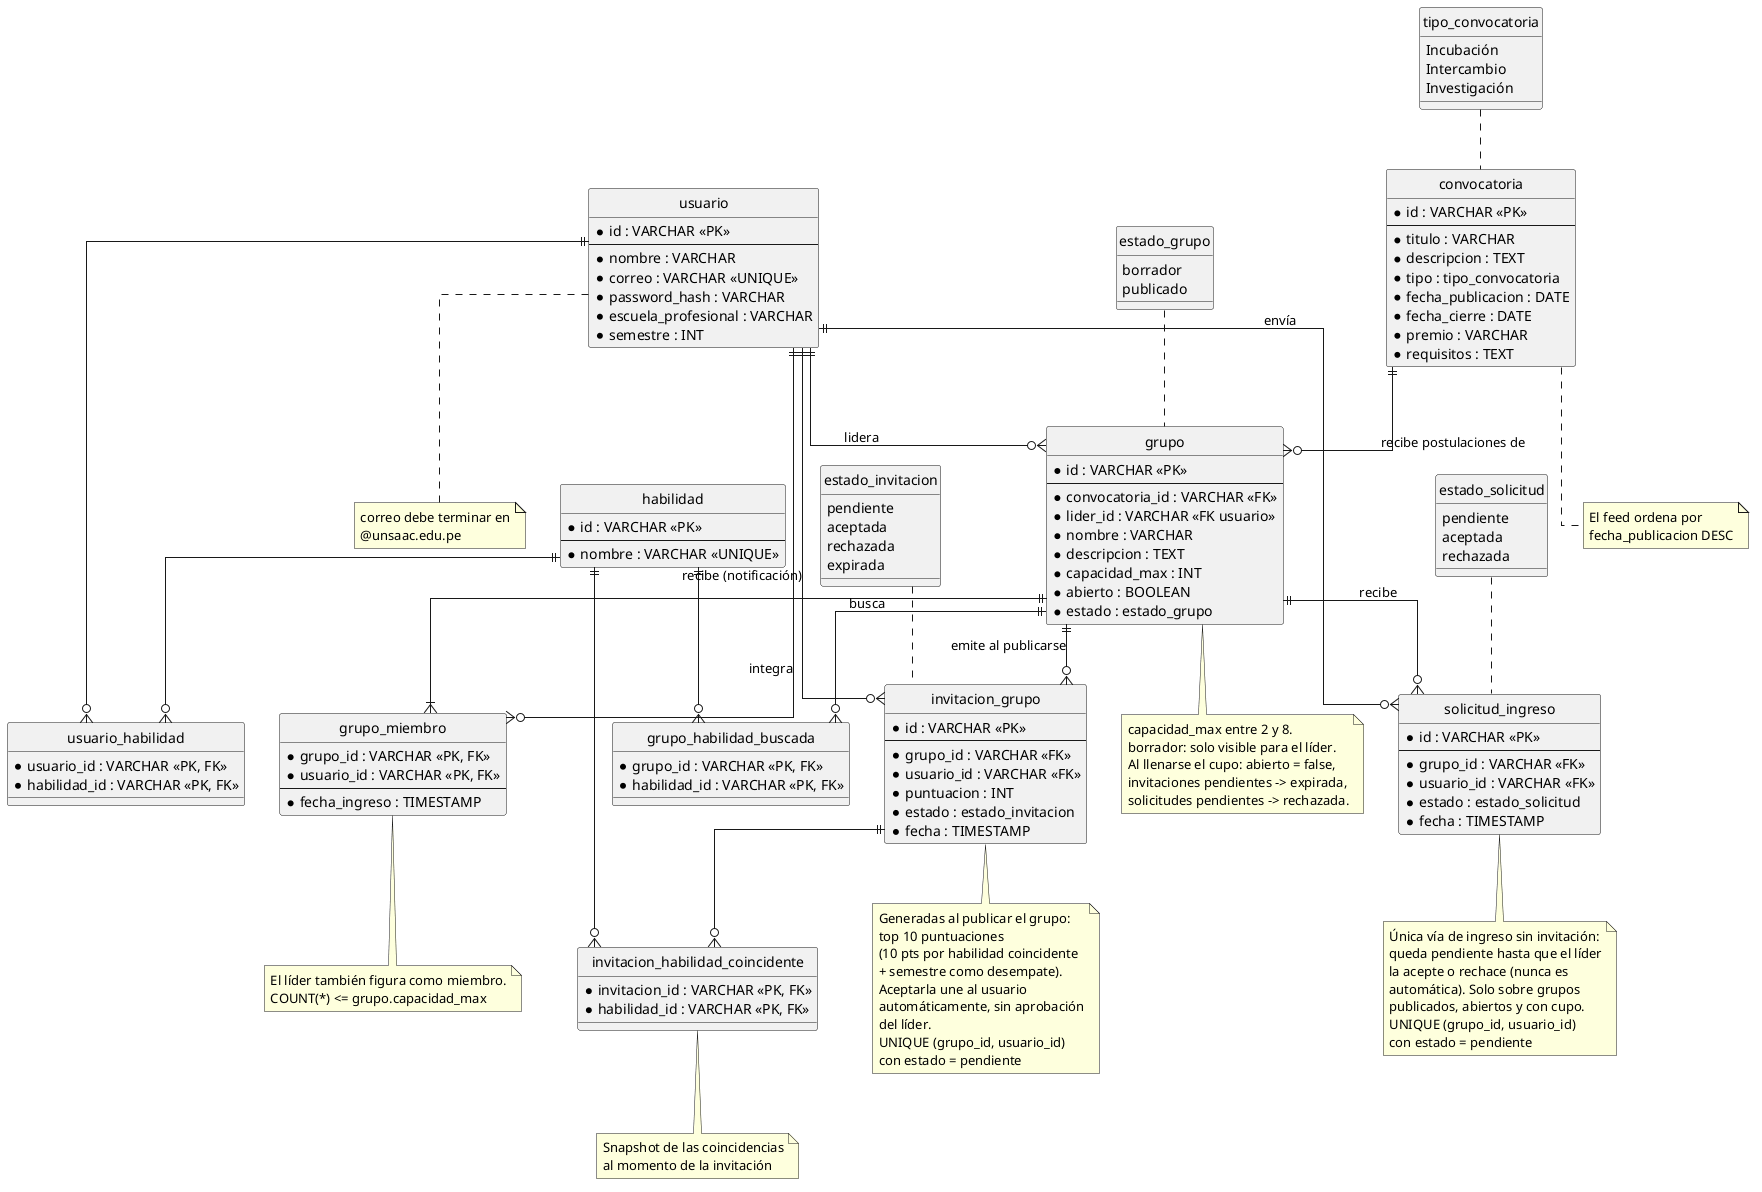
\includegraphics[width=\textwidth]{imagenes/modelo_datos.png}
\caption{Modelo lógico relacional del dominio de Yuyanna Hub}
\label{fig:modelo}
\end{figure}

\newpage
\section{Motor de Emparejamiento Automático}
\label{sec:matching}

\subsection{Modelo conceptual}
El emparejamiento se modela como el cruce entre la \textbf{oferta de competencias} de un estudiante y la \textbf{demanda de competencias} de un equipo en formación. Cada usuario $u$ posee un conjunto de habilidades etiquetadas $H_u = \{h_1, h_2, \dots, h_n\}$; cada grupo $g$ declara un conjunto de habilidades buscadas $B_g$, que representa explícitamente su déficit.

A diferencia de un emparejamiento simétrico entre personas, aquí el objeto emparejado es el \textbf{equipo}, y el evento que dispara el cálculo es la \textbf{publicación del grupo}: mientras el grupo está en estado \texttt{borrador} es privado y no genera ninguna notificación; al publicarse, el sistema busca activamente a quienes lo completan.

\subsection{Función de compatibilidad implementada}
Sea $M(u,g)$ el conjunto de habilidades buscadas por el grupo que el usuario efectivamente cubre:

\[
M(u,g) = \{\, b \in B_g \;\mid\; \exists\, h \in H_u : \; b \approx h \,\}
\]

donde $\approx$ denota la relación de coincidencia difusa definida en la sección~\ref{sec:coincidencia}. El puntaje de compatibilidad es entonces:

\[
\mathrm{Score}(u, g) \;=\; 10 \cdot \underbrace{|M(u,g)|}_{\text{habilidades cubiertas}} \;+\; \underbrace{\min\bigl(\mathrm{sem}(u),\, 9\bigr)}_{\text{criterio de desempate}}
\]

siendo $\mathrm{sem}(u)$ el semestre declarado por el usuario (0 si no lo declaró, por ejemplo un perfil externo).

\paragraph{Propiedad de ordenamiento.} La constante 10 y el recorte del semestre a 9 no son arbitrarios: garantizan que el puntaje ordene a los candidatos \textbf{lexicográficamente} por el par $(|M(u,g)|,\ \mathrm{sem}(u))$.

\emph{Demostración.} El término de desempate está acotado por $0 \le \min(\mathrm{sem}(u),9) \le 9 < 10$. Por lo tanto, si $|M(u_1,g)| > |M(u_2,g)|$, entonces $|M(u_1,g)| \ge |M(u_2,g)| + 1$ y
\[
\mathrm{Score}(u_1,g) \ge 10\,|M(u_2,g)| + 10 > 10\,|M(u_1',g)| + 9 \ge \mathrm{Score}(u_2,g),
\]
de modo que ninguna diferencia de semestre puede revertir una diferencia en el número de habilidades cubiertas. El semestre solo decide entre candidatos empatados en cobertura. $\square$

La consecuencia de diseño es intencional: \textbf{la cobertura del déficit manda; la antigüedad académica solo desempata}. Un estudiante de segundo semestre que cubre tres habilidades buscadas siempre se ordena por encima de uno de décimo que cubre dos.

\subsection{Coincidencia difusa de habilidades}
\label{sec:coincidencia}
Las habilidades son texto libre escrito por personas distintas, de modo que la igualdad exacta de cadenas produciría falsos negativos evidentes (``Python'' frente a ``python'', ``Diseño UX'' frente a ``diseno ux''). La relación $b \approx h$ se define en tres pasos:

\begin{enumerate}
    \item \textbf{Normalización:} ambas cadenas se recortan, se pasan a minúsculas y se les eliminan las tildes (\texttt{á}$\to$\texttt{a}, \texttt{é}$\to$\texttt{e}, \texttt{í}$\to$\texttt{i}, \texttt{ó}$\to$\texttt{o}, \texttt{ú}/\texttt{ü}$\to$\texttt{u}).
    \item \textbf{Igualdad:} si las cadenas normalizadas son idénticas, coinciden.
    \item \textbf{Contención con umbral:} si una contiene a la otra \emph{y} la cadena contenida tiene al menos 4 caracteres, también coinciden. Así ``Flutter'' coincide con ``Flutter avanzado'', mientras que el umbral de 4 caracteres evita que fragmentos como ``UX'' o ``IA'' disparen coincidencias espurias dentro de palabras no relacionadas.
\end{enumerate}

\subsection{Algoritmo de publicación y notificación}
El procedimiento completo, implementado en \texttt{GrupoService.publicarGrupo}, es el siguiente:

\begin{verbatim}
Entrada : grupo g (en estado borrador)
Salida  : g publicado + lista de invitaciones emitidas

1.  g.estado <- publicado ; persistir g
2.  si B_g = vacío  o  g está lleno : retornar sin invitaciones
3.  C <- directorio completo de usuarios  \  miembros actuales de g
4.  P <- vacío
5.  para cada candidato u en C:
6.        M <- habilidades de B_g cubiertas por u   (coincidencia difusa)
7.        si M = vacío : continuar          # no se notifica a quien no aporta
8.        P <- P + (u, 10*|M| + min(sem(u),9), M)
9.  ordenar P por puntaje descendente
10. para cada uno de los primeros 10 elementos de P:
11.       crear invitación pendiente con puntaje y coincidencias
\end{verbatim}

Tres decisiones merecen destacarse:

\begin{itemize}
    \item \textbf{Filtro estricto de relevancia (línea 7).} Un candidato sin ninguna habilidad coincidente \emph{nunca} es notificado, sin importar cuántos huecos tenga el grupo. Esto cumple el criterio de ``umbral mínimo'' del diseño original: la bandeja de invitaciones no se contamina con ruido.
    \item \textbf{Tope de diez invitaciones} (\texttt{GrupoService.maxInvitaciones}). Acota tanto el costo de escritura en Firestore como la presión social sobre el directorio: publicar un grupo no genera una notificación masiva al campus.
    \item \textbf{Instantánea del cálculo.} El puntaje y las habilidades coincidentes se guardan en la invitación, no se recalculan al leerla.
\end{itemize}

\paragraph{Complejidad.} El cálculo es $O(|C| \cdot |B_g| \cdot |H_u|)$ comparaciones de cadenas cortas, ejecutado una única vez por publicación de grupo y sobre un directorio del orden de los miles de perfiles: perfectamente asumible en el cliente. Su costo dominante no es el cómputo sino la lectura del directorio (una consulta) y la escritura de hasta diez invitaciones.

\subsection{Ciclo de vida del ingreso a un equipo}
El emparejamiento produce invitaciones, pero el ingreso efectivo admite dos vías, deliberadamente asimétricas:

\begin{table}[htbp]
\centering
\caption{Vías de ingreso a un grupo}
\begin{tabular}{L{3.3cm}L{4.6cm}L{5.6cm}}
\toprule
\textbf{Vía} & \textbf{Quién la origina} & \textbf{Quién decide} \\
\midrule
Invitación & El sistema, al publicarse el grupo & \textbf{El invitado}: aceptar lo une de inmediato, porque la invitación ya lo pre-aprobó. \\
Solicitud de ingreso & El propio usuario, desde la vista de grupos & \textbf{El líder}: acepta o rechaza; nunca es automática. \\
Alta directa & El líder, desde su grupo & \textbf{El líder}, eligiendo del directorio. \\
\bottomrule
\end{tabular}
\end{table}

Al completarse el cupo (\texttt{integrantes = capacidad\_max}) se dispara un \textbf{cierre en cascada}: el grupo pasa a \texttt{abierto = false}, todas sus invitaciones pendientes se marcan \texttt{expirada} y todas sus solicitudes pendientes se marcan \texttt{rechazada}. Simétricamente, cuando un usuario entra al grupo por una vía, sus pendientes por la otra vía se resuelven para que no queden notificaciones huérfanas. Esta cascada es la razón técnica del compromiso de seguridad descrito en la sección~\ref{sec:tradeoff}.

\newpage
\section{Seguridad y Control de Acceso}
\label{sec:seguridad}

\subsection{Autenticación}
La autenticación se delega íntegramente a \textbf{Firebase Authentication} con proveedor de correo y contraseña. La aplicación \emph{nunca} recibe, transporta ni almacena contraseñas: Firebase gestiona el almacenamiento con derivación de clave (\emph{scrypt}) y expone únicamente el \texttt{uid}. Al registrarse, el usuario recibe un correo de verificación; existe además el flujo de restablecimiento de contraseña desde la pantalla de inicio de sesión.

El perfil se escribe en \texttt{usuarios/\{uid\}} y se cachea localmente en \texttt{LocalSessionManager} (\texttt{shared\_preferences}), de modo que el arranque de la aplicación resuelve la sesión sin una lectura remota. La pantalla de bienvenida (\texttt{SplashScreen}) consulta esa bandera local tras 2.5 segundos y deriva al feed o al inicio de sesión.

\subsection{Identidad institucional}
La constante \texttt{Usuario.dominioUnsaac} (\texttt{@unsaac.edu.pe}) y la propiedad derivada \texttt{esUnsaac} determinan si una cuenta pertenece a la comunidad universitaria, lo que se refleja en el perfil con la insignia \emph{Estudiante UNSAAC}. Se trata de una \textbf{distinción, no de una restricción}: la justificación se detalla en la sección~\ref{sec:limitaciones}.

\subsection{Roles de administración}
Los roles viven en la colección \texttt{admins}, donde \emph{la existencia del documento es el rol}:

\begin{itemize}
    \item \texttt{admin} --- administrador completo. Accede al panel de administración y puede crear, editar y eliminar eventos, ver el directorio y los grupos, y promover o degradar a otros administradores.
    \item \texttt{admin\_paqarina} --- gestor de la incubadora. Puede publicar eventos, pero no accede al panel ni edita o elimina lo publicado por otros.
\end{itemize}

El \textbf{problema del primer administrador} (nadie puede promover al primero si aún no hay ninguno) se resuelve con un \emph{bootstrap} por lista de correos fundadores: si un usuario cuyo correo figura en \texttt{AdminService.correosFundadores} inicia sesión y todavía no tiene documento en \texttt{admins}, la aplicación se lo crea con rol \texttt{admin} al cargar la pantalla principal. La misma lista está replicada en la función \texttt{esFundador()} de \texttt{firestore.rules}; ambas \textbf{deben mantenerse sincronizadas}, pues la regla del servidor es la que realmente autoriza la operación.

\subsection{Reglas de seguridad del servidor}
La autorización no se confía al cliente. \texttt{firestore.rules} define las funciones \texttt{estaAutenticado()}, \texttt{esAdmin()}, \texttt{tieneRolAdmin()} y \texttt{esFundador()}, y con ellas:

\begin{table}[htbp]
\centering
\caption{Permisos por colección según las Security Rules}
\begin{tabular}{L{2.6cm}L{2.6cm}L{8.3cm}}
\toprule
\textbf{Colección} & \textbf{Lectura} & \textbf{Escritura} \\
\midrule
\texttt{usuarios} & Autenticado & Solo el propio usuario sobre su documento (\texttt{uid} coincidente). Borrado prohibido. \\
\texttt{convocatorias} & Autenticado & Crear: cualquier rol admin. Editar y eliminar: solo \texttt{admin} completo. \\
\texttt{admins} & Admin, o el propio interesado & Crear: un fundador sobre sí mismo, o un admin sobre otros. Cambiar rol y eliminar: solo admin. \\
\texttt{grupos} & Autenticado & Crear: solo si \texttt{lider\_id} es el propio \texttt{uid}. Eliminar: líder o admin. Actualizar: cualquier autenticado. \\
\texttt{invitaciones}, \texttt{solicitudes} & Autenticado & Cualquier autenticado. \\
\bottomrule
\end{tabular}
\end{table}

\subsection{Compromiso documentado sobre la escritura de equipos}
\label{sec:tradeoff}
Las tres últimas filas de la tabla anterior son deliberadamente permisivas y constituyen el principal compromiso técnico del proyecto. La causa es estructural: \textbf{sin Cloud Functions} (no disponibles en el plan gratuito \emph{Spark}), la lógica de equipos corre en el cliente, y esa lógica \textbf{toca documentos de otros usuarios}. Cuando un estudiante acepta la última plaza de un grupo, su dispositivo debe expirar las invitaciones pendientes \emph{de terceros} y rechazar las solicitudes \emph{de terceros}. Ninguna regla que restrinja la escritura a ``dueño o líder'' permitiría esa cascada.

Se optó por hacer el compromiso \textbf{explícito y acotado} en lugar de disimularlo: está comentado en el propio archivo de reglas, se limita a tres colecciones que no contienen credenciales ni datos sensibles, y todas las operaciones siguen exigiendo usuario autenticado. La ruta de remediación es conocida y está descrita en la sección~\ref{sec:futuro}: migrar la cascada a Cloud Functions bajo el plan \emph{Blaze} y endurecer las reglas a ``dueño o líder'', ejecutando el cierre dentro de una transacción.

\subsection{Gestión de multimedia}
Firebase Storage tampoco está disponible en el plan gratuito, por lo que el material audiovisual de los eventos se resolvió con un \textbf{Cloudflare Worker} propio sobre un \emph{bucket} R2:

\begin{itemize}
    \item \texttt{POST /upload} exige un \emph{ID token} de Firebase en la cabecera \texttt{Authorization}, verifica su firma RS256 contra las claves públicas de Google y comprueba el rol administrador del emisor, sanea el nombre del archivo (solo caracteres alfanuméricos, punto, guion y guion bajo; máximo 80 caracteres), le antepone marca de tiempo y un UUID parcial para evitar colisiones, lo guarda en R2 y devuelve la URL pública.
    \item \texttt{GET /file/<clave>} entrega el archivo con \texttt{Cache-Control} inmutable de un año y \textbf{soporte del encabezado \texttt{Range}} (respuestas 206), requisito para que el video del feed pueda buscarse y reproducirse progresivamente.
\end{itemize}

En Firestore solo se persiste la URL (\texttt{imagen\_url}, \texttt{video\_url}); el binario nunca entra en la base de datos.

\newpage
\section{Diseño de Interfaz y Flujo de Navegación}

\subsection{Sistema de diseño}
Todo el estilo está centralizado en \texttt{lib/theme/}, y ninguna pantalla codifica colores ni estilos de texto directamente. La paleta es institucional (rojo, azul y dorado de la UNSAAC) sobre un fondo de papel cálido:

\begin{table}[htbp]
\centering
\caption{Paleta institucional (extracto de \texttt{AppColors})}
\begin{tabular}{L{3.4cm}L{2.6cm}L{7.5cm}}
\toprule
\textbf{Rol} & \textbf{Valor} & \textbf{Uso} \\
\midrule
\texttt{paper} & \texttt{\#FAF7F2} & Fondo general de la aplicación. \\
\texttt{ink} / \texttt{inkSecondary} & \texttt{\#1F1A2E} / \texttt{\#6B6478} & Texto principal y secundario. \\
\texttt{red} / \texttt{redFill} / \texttt{redDeep} & \texttt{\#A6213B} \dots & Acción primaria, eventos de investigación. \\
\texttt{blue} / \texttt{blueFill} / \texttt{blueDeep} & \texttt{\#1F4E8C} \dots & Hackatones e intercambio. \\
\texttt{gold} / \texttt{goldFill} / \texttt{goldDeep} & \texttt{\#A87410} \dots & Incubación y preincubación. \\
\bottomrule
\end{tabular}
\end{table}

La clase auxiliar \texttt{TipoConvocatoria} traduce el tipo textual de un evento a su color y su degradado, de modo que el código cromático es consistente en el feed, las tarjetas y las etiquetas. El tema es Material 3 en variante clara únicamente, con tipografía servida por \texttt{google\_fonts} y animaciones de entrada con \texttt{flutter\_animate}.

\subsection{Flujo de navegación}
La navegación es explícita y sin rutas nombradas:

\begin{verbatim}
SplashScreen (2.5 s, lee la sesión local)
     |-- sin sesión --> LoginScreen <--> RegisterScreen
     `-- con sesión --> HomeScreen
                          |
                          |-- IndexedStack de 3 pestañas (MenuWidget inferior)
                          |     |-- 0. Feed vertical de convocatorias
                          |     |-- 1. Panel de administración   (solo admin)
                          |     `-- 2. Perfil --> EditarPerfilScreen
                          |
                          |-- NotificacionesScreen   (campana + contador)
                          |-- CrearConvocatoriaScreen (solo roles admin)
                          `-- GruposScreen (de una convocatoria)
                                 |-- CrearGrupoScreen
                                 `-- MisGruposScreen
\end{verbatim}

La pantalla principal mantiene las tres pestañas vivas en un \texttt{IndexedStack} (el estado del feed no se pierde al visitar el perfil) y empuja las pantallas de detalle con \texttt{Navigator.push}. La pestaña de administración solo aparece para el rol \texttt{admin} completo.

\subsection{El feed de convocatorias}
La decisión de interfaz más característica del proyecto es presentar las convocatorias como un \textbf{\texttt{PageView} vertical a pantalla completa}, con el lenguaje visual de las plataformas de video corto que el público objetivo ya domina, en lugar de una lista de tarjetas administrativas. Cada página incluye:

\begin{itemize}
    \item La imagen o el video del evento como fondo. La imagen se ajusta al ancho completo sin recortar los lados, y el espacio sobrante se rellena con un degradado derivado del \textbf{color dominante de la propia imagen}, calculado con \texttt{palette\_generator}; mientras se calcula, se muestra el degradado del tipo de evento.
    \item Título, tipo, fecha de cierre, premio y requisitos, con la descripción truncada y un enlace ``Leer más'' que solo aparece si el texto no cabe completo.
    \item Un riel lateral de acciones y el acceso directo a los grupos de esa convocatoria.
    \item Un \textbf{modo inmersivo}: el doble toque oculta todos los elementos superpuestos y deja únicamente la imagen; otro doble toque los restituye.
\end{itemize}

La barra superior muestra el contador de invitaciones pendientes, obtenido mediante \texttt{getInvitacionesParaUsuario}, que actúa como notificación interna a falta de mensajería \emph{push}.

\subsection{Pantallas de formación de equipos}
\begin{itemize}
    \item \textbf{\texttt{CrearGrupoScreen}} --- recibe la convocatoria ya seleccionada y solicita nombre, descripción, capacidad máxima (validada entre 2 y 8 integrantes), integrantes iniciales tomados del directorio mediante \texttt{selector\_usuario}, y las habilidades buscadas mediante \texttt{selector\_habilidades}. El grupo nace en estado \texttt{borrador}.
    \item \textbf{\texttt{MisGruposScreen}} --- lista los grupos que el usuario lidera, distingue borradores de publicados y ofrece la acción de publicar, que es la que dispara el motor de emparejamiento.
    \item \textbf{\texttt{GruposScreen}} --- muestra los grupos publicados de una convocatoria (más los borradores propios), permite solicitar el ingreso y, al líder, resolver las solicitudes recibidas.
    \item \textbf{\texttt{NotificacionesScreen}} --- bandeja de invitaciones pendientes; cada tarjeta indica el grupo, el puntaje y \emph{qué habilidades} motivaron la invitación, con las acciones de unirse o rechazar.
\end{itemize}

\subsection{Panel de administración}
\texttt{AdminPanelScreen} organiza la gestión en cuatro pestañas: \textbf{Eventos} (alta, edición y eliminación de convocatorias), \textbf{Usuarios} (directorio con la etiqueta de rol de cada uno), \textbf{Grupos} (todos los grupos creados, con eliminación) y \textbf{Admins} (promoción por correo, cambio de rol \texttt{admin} $\leftrightarrow$ \texttt{admin\_paqarina} y revocación).

\subsection{Capturas de pantalla de la aplicación}

A continuación, se presentan las capturas de pantalla de las principales interfaces de la aplicación Yuyanna Hub.

\begin{figure}[htbp]
    \centering
    \begin{minipage}{0.31\textwidth}
        \centering
        
\includegraphics[width=\linewidth]{app_imagenes/Login.jpeg}
        \caption{Inicio de sesión}
    \end{minipage}\hfill
    \begin{minipage}{0.31\textwidth}
        \centering
        
\includegraphics[width=\linewidth]{app_imagenes/Register.jpeg}
        \caption{Registro}
    \end{minipage}\hfill
    \begin{minipage}{0.31\textwidth}
        \centering
        
\includegraphics[width=\linewidth]{app_imagenes/Inicio.jpeg}
        \caption{Feed de convocatorias}
    \end{minipage}
\end{figure}

\begin{figure}[htbp]
    \centering
    \begin{minipage}{0.31\textwidth}
        \centering
        
\includegraphics[width=\linewidth]{app_imagenes/Grupos.jpeg}
        \caption{Grupos}
    \end{minipage}\hfill
    \begin{minipage}{0.31\textwidth}
        \centering
        
\includegraphics[width=\linewidth]{app_imagenes/Crear_grupo.jpeg}
        \caption{Crear grupo}
    \end{minipage}\hfill
    \begin{minipage}{0.31\textwidth}
        \centering
        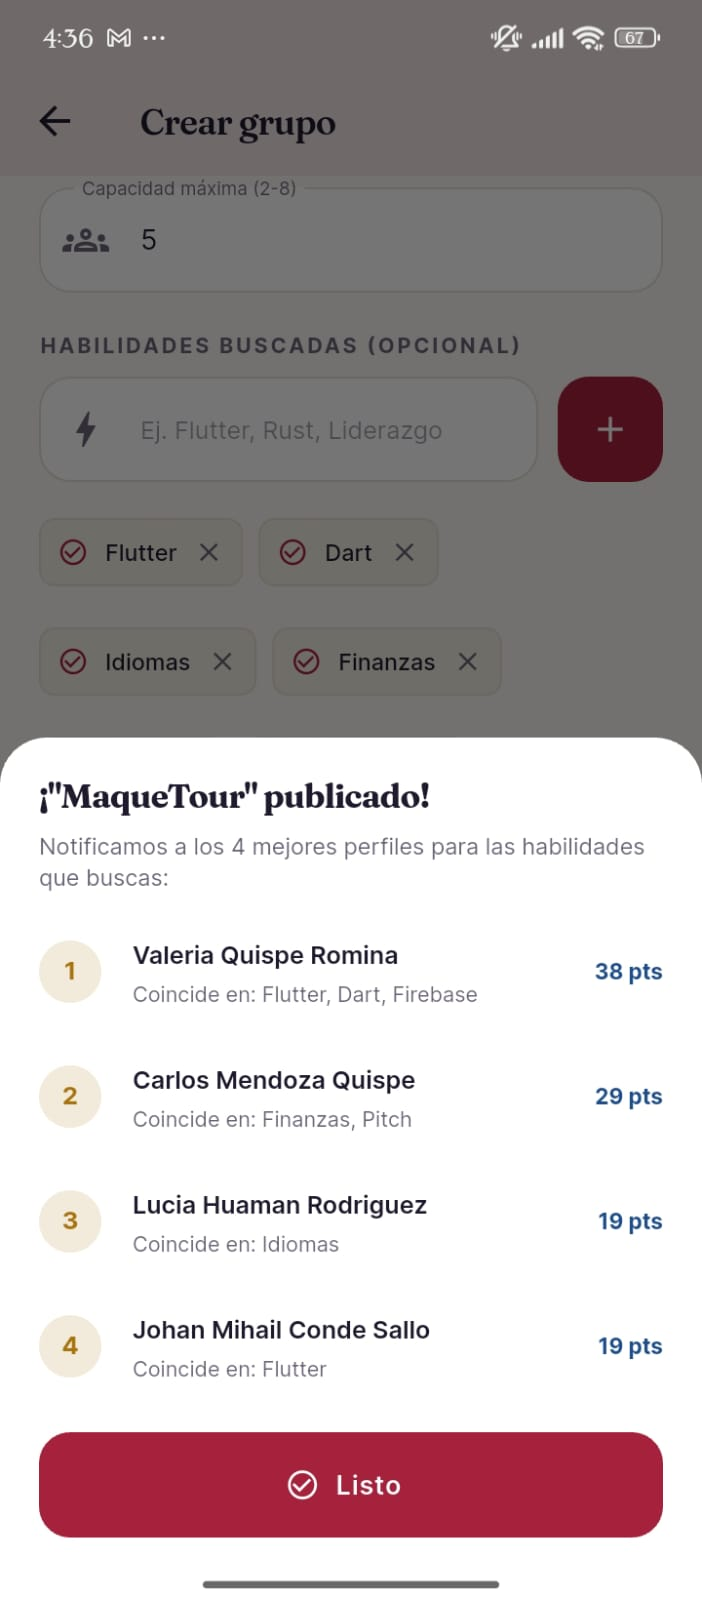
\includegraphics[width=\linewidth]{app_imagenes/Puntuaciones_crear_grupo.jpeg}
        \caption{Emparejamiento}
    \end{minipage}
\end{figure}

\begin{figure}[htbp]
    \centering
    \begin{minipage}{0.31\textwidth}
        \centering
        
\includegraphics[width=\linewidth]{app_imagenes/Notificacion_invitacion_grupo.jpeg}
        \caption{Invitaciones}
    \end{minipage}\hfill
    \begin{minipage}{0.31\textwidth}
        \centering
        
\includegraphics[width=\linewidth]{app_imagenes/Perfil_estudiante.jpeg}
        \caption{Perfil estudiante}
    \end{minipage}\hfill
    \begin{minipage}{0.31\textwidth}
        \centering
        
\includegraphics[width=\linewidth]{app_imagenes/Editar_perfil.jpeg}
        \caption{Editar perfil}
    \end{minipage}
\end{figure}

\begin{figure}[htbp]
    \centering
    \begin{minipage}{0.31\textwidth}
        \centering
        
\includegraphics[width=\linewidth]{app_imagenes/Perfil_administrador.jpeg}
        \caption{Panel Admin}
    \end{minipage}\hfill
    \begin{minipage}{0.31\textwidth}
        \centering
        
\includegraphics[width=\linewidth]{app_imagenes/Publicar_evento.jpeg}
        \caption{Publicar Evento}
    \end{minipage}\hfill
    \begin{minipage}{0.31\textwidth}
        \centering
        
\includegraphics[width=\linewidth]{app_imagenes/Vista_superadmin.jpeg}
        \caption{Superadmin}
    \end{minipage}
\end{figure}

\newpage
\section{Pruebas y Verificación}

\subsection{Estrategia}
La estrategia de pruebas concentra el esfuerzo donde está el riesgo: la \textbf{lógica de dominio} de formación de equipos y emparejamiento, que es la única parte del sistema con reglas de negocio propias. Las pruebas se ejecutan contra \texttt{fake\_cloud\_firestore}, un doble en memoria de Firestore, de modo que verifican el comportamiento real del servicio ---incluidas sus consultas y escrituras--- sin tocar la base de datos de producción ni requerir conexión. Un segundo bloque de pruebas recorre el camino completo de la aplicación ---alta de usuarios con \texttt{AuthService.registrar}, creación y publicación del grupo, y lectura de la bandeja de invitaciones--- para descartar desajustes entre lo que el registro escribe y lo que el motor de emparejamiento lee.

\subsection{Casos de prueba automatizados}
\begin{longtable}{L{3.4cm}L{10.4cm}}
\caption{Suite de pruebas automatizadas}\label{tab:tests}\\
\toprule
\textbf{Archivo} & \textbf{Caso verificado} \\
\midrule
\endfirsthead
\toprule
\textbf{Archivo} & \textbf{Caso verificado} \\
\midrule
\endhead
\bottomrule
\endfoot
\texttt{grupo\_service\_test} & El grupo se crea en estado \texttt{borrador}, con el líder registrado como miembro y los integrantes iniciales incorporados. \\
\texttt{grupo\_service\_test} & Al publicar, solo se notifica a perfiles con al menos una habilidad coincidente; las invitaciones salen ordenadas por puntaje descendente y no superan el máximo de diez. El perfil sin coincidencias no recibe invitación. \\
\texttt{grupo\_service\_test} & Un invitado que acepta se incorpora automáticamente al grupo, sin intervención del líder. \\
\texttt{grupo\_service\_test} & Una solicitud de ingreso permanece pendiente hasta que el líder la resuelve; nunca produce un ingreso automático. \\
\texttt{grupo\_service\_test} & Al llenarse el cupo, el grupo se cierra y las invitaciones y solicitudes pendientes quedan expiradas o rechazadas (cierre en cascada). \\
\texttt{habilidades\_test} & El catálogo de habilidades no está vacío; \texttt{agregarHabilidad} inserta nuevas entradas y evita duplicados sin distinguir mayúsculas; el texto separado por comas se procesa elemento por elemento; la búsqueda filtra correctamente. \\
\texttt{habilidades\_test} & El \emph{widget} \texttt{SelectorHabilidades} renderiza las habilidades seleccionadas como \emph{chips} y las elimina una a una al tocar su ícono de cierre. \\
\texttt{widget\_test} & Prueba de humo de arranque: la pantalla de bienvenida muestra el nombre de la aplicación (adelantando el temporizador de 2.5 s para no dejar temporizadores pendientes). \\
\texttt{diagnostico\_matching\_test} & Recorrido de extremo a extremo por el camino real de la aplicación: tres estudiantes se dan de alta con \texttt{AuthService.registrar}, el líder crea y publica un grupo, y la única candidata compatible recibe la invitación en la bandeja que lee \texttt{NotificacionesScreen}. \\
\texttt{diagnostico\_matching\_test} & Un grupo publicado sin habilidades buscadas no emite ninguna invitación (el motor no tiene criterio con el cual puntuar). \\
\texttt{diagnostico\_matching\_test} & Un grupo que queda en \texttt{borrador} no genera invitaciones, aunque exista un perfil que coincida por completo. \\
\end{longtable}

\subsection{Resultados de la verificación}
\begin{table}[htbp]
\centering
\caption{Resultados de las herramientas de verificación}
\begin{tabular}{L{4.6cm}L{4.0cm}L{5.0cm}}
\toprule
\textbf{Herramienta} & \textbf{Comando} & \textbf{Resultado} \\
\midrule
Analizador estático & \texttt{flutter analyze} & \textbf{Sin observaciones} (\emph{No issues found}). \\
Pruebas automatizadas & \texttt{flutter test} & \textbf{15 de 15 pruebas superadas.} \\
\bottomrule
\end{tabular}
\end{table}

\subsection{Métricas del producto}
\begin{table}[htbp]
\centering
\caption{Métricas del código fuente}
\begin{tabular}{L{7.5cm}L{5.5cm}}
\toprule
\textbf{Métrica} & \textbf{Valor} \\
\midrule
Archivos fuente Dart (\texttt{lib/} y \texttt{test/}) & 39 \\
Líneas de código Dart & $\approx$ 9\,770 \\
Modelos de dominio & 6 \\
Servicios & 6 \\
Pantallas & 12 \\
\emph{Widgets} reutilizables & 6 \\
Colecciones de Firestore & 6 \\
Pruebas automatizadas & 12 \\
Plataformas objetivo & Android y web \\
\bottomrule
\end{tabular}
\end{table}

\subsection{Verificación manual}
Además de la suite automatizada, se validaron manualmente los recorridos que dependen de servicios externos y no son reproducibles con dobles: registro con verificación de correo, restablecimiento de contraseña, \emph{bootstrap} del administrador fundador, publicación de un evento con imagen y video (subida al Worker de Cloudflare y reproducción con búsqueda dentro del video), y el ciclo completo de publicación de grupo con recepción de la invitación en una segunda cuenta.

\newpage
\section{Trazabilidad: Planificado frente a Alcanzado}
\label{sec:trazabilidad}

\begin{longtable}{L{1.5cm}L{4.1cm}L{2.9cm}L{5.0cm}}
\caption{Cumplimiento de los requerimientos funcionales}\label{tab:traza-rf}\\
\toprule
\textbf{Código} & \textbf{Requerimiento} & \textbf{Estado} & \textbf{Observación} \\
\midrule
\endfirsthead
\toprule
\textbf{Código} & \textbf{Requerimiento} & \textbf{Estado} & \textbf{Observación} \\
\midrule
\endhead
\bottomrule
\endfoot
RF-01 & Autenticación de cuentas & \parcial & Implementada con correo y contraseña, verificación de correo y restablecimiento. Se sustituyó el código OTP planificado y se relajó la restricción de dominio (véase~\ref{sec:desviaciones}). \\
RF-02 & Perfil de habilidades & \impl & Incluye tipo de perfil estudiante/externo. No se implementó el enlace a portafolios externos. \\
RF-03 & Mapeo de convocatorias & \impl & Alta, edición y eliminación desde el panel, con imagen y video. Los tipos activos son Hackatón, Incubación y Pre incubación. \\
RF-04 & Publicación de equipos y déficit & \impl & El déficit se declara como conjunto de habilidades buscadas, no como plazas nominadas con rol y escuela. \\
RF-05 & Motor de emparejamiento & \parcial & Implementada la dirección \emph{equipo $\rightarrow$ candidatos} (invitaciones automáticas al publicar). La recomendación inversa ranqueada \emph{estudiante $\rightarrow$ equipos} quedó pendiente. \\
RF-06 & Postulación y aprobación & \impl & Ambas vías (invitación y solicitud) más el cierre automático en cascada. \\
RF-07 & Bandeja de notificaciones & \parcial & Bandeja interna con contador, funcional. No hay notificaciones \emph{push} (requieren FCM y plan de pago). \\
RF-08 & Panel de administración & \impl & Cuatro pestañas con dos roles diferenciados. \\
RF-09 & Gestión de multimedia & \impl & Worker de Cloudflare sobre R2, con soporte de \texttt{Range} para video. \\
\end{longtable}

\begin{longtable}{L{1.7cm}L{4.3cm}L{2.7cm}L{4.8cm}}
\caption{Cumplimiento de los requerimientos no funcionales}\label{tab:traza-rnf}\\
\toprule
\textbf{Código} & \textbf{Requerimiento} & \textbf{Estado} & \textbf{Observación} \\
\midrule
\endfirsthead
\toprule
\textbf{Código} & \textbf{Requerimiento} & \textbf{Estado} & \textbf{Observación} \\
\midrule
\endhead
\bottomrule
\endfoot
RNF-01 & Multiplataforma & \impl & Android y web desde una sola base de código. iOS quedó fuera del alcance (requiere equipo y cuenta de desarrollador Apple). \\
RNF-02 & Costo de operación & \impl & Opera íntegramente sobre planes gratuitos. \\
RNF-03 & Eficiencia de lectura & \impl & Miembros desnormalizados (una lectura por grupo) y consultas de un solo campo (cero índices compuestos). \\
RNF-04 & Seguridad y control de acceso & \parcial & Reglas del servidor activas y roles reforzados, con el compromiso explícito de escritura sobre grupos, invitaciones y solicitudes (\ref{sec:tradeoff}). \\
RNF-05 & Persistencia de sesión & \impl & Caché local del perfil en \texttt{shared\_preferences}. \\
RNF-06 & Idioma y consistencia & \impl & Dominio, interfaz e identificadores en español. \\
RNF-07 & Calidad de código & \impl & \texttt{flutter analyze} sin observaciones; 15 pruebas en verde. \\
\end{longtable}

\subsection{Desviaciones respecto del plan original y su justificación}
\label{sec:desviaciones}

\begin{enumerate}
    \item \textbf{Autenticación por contraseña en lugar de código OTP.} El envío de códigos de un solo uso exige una función de servidor que genere, almacene y valide el código, además de un proveedor de correo transaccional; ambas cosas están fuera del plan gratuito. Firebase Authentication ofrece, sin costo, un flujo equivalente en garantías de posesión del buzón (verificación de correo y restablecimiento por enlace firmado) con una implementación notablemente más simple y auditada.

    \item \textbf{El dominio institucional distingue, no restringe.} El plan original bloqueaba el acceso a cuentas ajenas a \texttt{@unsaac.edu.pe}. Durante el desarrollo se identificó que los usuarios secundarios legítimos ---mentores externos, egresados sin correo institucional vigente y los propios gestores de la incubadora--- quedaban excluidos por esa regla. La solución adoptada conserva la señal de confianza sin perder cobertura: cualquiera puede registrarse, pero solo las cuentas del dominio exhiben la insignia \emph{Estudiante UNSAAC}, y el modelo de perfil admite explícitamente el tipo \emph{externo} con su campo de ocupación.

    \item \textbf{Backend gestionado en lugar de API propia en Rust/Axum.} El plan contemplaba un servicio propio. Se optó por Firebase para eliminar el costo de operación y de despliegue de un servidor durante el piloto, y para concentrar el esfuerzo del semestre en el dominio (emparejamiento y formación de equipos) en lugar de en infraestructura. El costo de esta decisión está documentado en~\ref{sec:tradeoff}.

    \item \textbf{Función de compatibilidad aditiva en lugar de similitud de Jaccard ponderada.} La formulación inicial combinaba similitud de Jaccard, coincidencia de escuela y un término de diversidad, con pesos $\alpha, \beta, \gamma$. Se reemplazó por la función descrita en la sección~\ref{sec:matching} por tres razones concretas: (a) el denominador de Jaccard $|H_u \cup H_v|$ \textbf{penaliza a los perfiles más completos} ---un estudiante que declara veinte habilidades obtiene menor similitud que uno que declara tres, aun cubriendo el mismo déficit---, lo que es exactamente el comportamiento contrario al deseado; (b) los pesos $\alpha, \beta, \gamma$ no eran calibrables sin datos históricos de uso, de los que el piloto aún carece; y (c) la función adoptada es \emph{explicable}: la invitación puede mostrar literalmente qué habilidades motivaron el puntaje, lo que la formulación fraccionaria no permite comunicar con claridad. El término de diversidad multidisciplinaria quedó registrado como trabajo futuro (\ref{sec:futuro}).

    \item \textbf{Déficit expresado como habilidades y no como plazas nominadas.} Modelar cada vacante con rol, escuela deseada y habilidades habría multiplicado la complejidad del formulario de creación de grupo, que es el punto de mayor fricción del recorrido. Se optó por un único conjunto de habilidades buscadas a nivel de equipo, que preserva la capacidad de emparejar sin exigir al líder un diseño organizacional previo.
\end{enumerate}

\newpage
\section{Limitaciones Conocidas}
\label{sec:limitaciones}

Se documentan de manera explícita las limitaciones del estado actual, por honestidad técnica y para orientar el trabajo posterior:

\begin{enumerate}
    \item \textbf{Escritura permisiva en tres colecciones.} Cualquier usuario autenticado puede escribir en \texttt{grupos}, \texttt{invitaciones} y \texttt{solicitudes}. Es el compromiso analizado en~\ref{sec:tradeoff}, aceptable para un piloto controlado e inaceptable para una operación abierta y prolongada.

    \item \textbf{Ausencia de transacciones.} El cierre en cascada al llenarse un grupo se ejecuta como una secuencia de escrituras independientes desde el cliente. Dos usuarios que acepten la última plaza simultáneamente podrían, en el peor caso, exceder la capacidad declarada. La solución correcta es una transacción de Firestore o, mejor, una Cloud Function.

    \item \textbf{Verificación de rol en cada subida.} El Worker consulta \texttt{admins/\{uid\}} en Firestore por cada archivo, lo que agrega una petición de red a la latencia de la subida. Para el volumen del piloto es irrelevante; a escala convendría trasladar el rol a un \emph{custom claim} del propio ID token, que se verifica sin salir del Worker.

    \item \textbf{Lista de fundadores duplicada.} Los correos fundadores están escritos tanto en \texttt{AdminService} como en \texttt{firestore.rules}; una divergencia entre ambos rompería el \emph{bootstrap} del primer administrador de forma silenciosa.

    \item \textbf{Emparejamiento como evento puntual.} El cálculo ocurre una sola vez, al publicar el grupo. Un usuario que se registra o que amplía sus habilidades después de esa publicación no será considerado, aunque sea el candidato ideal.

    \item \textbf{Directorio completo en memoria.} \texttt{getUsuarios()} descarga todos los perfiles para puntuarlos. Es adecuado para el orden de magnitud del piloto, pero no escala a decenas de miles de usuarios ni al presupuesto de lecturas del plan gratuito.

    \item \textbf{Sin notificaciones \emph{push}.} El contador de la barra superior solo se actualiza cuando la aplicación está abierta; una invitación puede pasar inadvertida hasta el siguiente ingreso.

    \item \textbf{Habilidades como texto libre.} El catálogo es un conjunto en memoria que cada instalación amplía localmente; no se sincroniza entre dispositivos, de modo que la coincidencia difusa carga con el peso de las variantes ortográficas.

    \item \textbf{Nombre engañoso de un archivo.} \texttt{lib/database/sqlite\_helper.dart} no contiene SQLite, sino el gestor de sesión sobre \texttt{shared\_preferences}; el nombre sobrevive de una etapa anterior del diseño.
\end{enumerate}

\newpage
\section{Trabajo Futuro}
\label{sec:futuro}

\begin{enumerate}
    \item \textbf{Migrar la lógica de equipos a Cloud Functions (plan \emph{Blaze}).} Es la mejora de mayor impacto: permitiría endurecer las reglas a ``dueño o líder'', ejecutar el cierre en cascada dentro de una transacción y eliminar simultáneamente las limitaciones 1 y 2.

    \item \textbf{Recomendación inversa (estudiante $\rightarrow$ equipos).} Completar el RF-05 con la vista ``equipos que te necesitan'', reutilizando la misma función de compatibilidad recorrida en sentido contrario sobre los grupos publicados y abiertos de las convocatorias vigentes.

    \item \textbf{Reemparejamiento incremental.} Recalcular las invitaciones cuando un usuario nuevo se registra o actualiza sus habilidades, mientras existan grupos publicados con plazas y déficit sin cubrir.

    \item \textbf{Incorporar el término de diversidad multidisciplinaria.} Añadir una bonificación por escuela profesional aún no representada en el equipo, respetando la propiedad de ordenamiento lexicográfico (un peso estrictamente menor que el paso de 10 puntos por habilidad), de manera que la diversidad desempate sin desplazar a la cobertura del déficit.

    \item \textbf{Notificaciones \emph{push} con Firebase Cloud Messaging}, para que una invitación llegue al dispositivo aunque la aplicación esté cerrada.

    \item \textbf{Catálogo de habilidades compartido en Firestore}, con normalización y fusión de sinónimos administrada desde el panel, reduciendo la dependencia de la coincidencia difusa.

    \item \textbf{Autorización real del Worker de subida} mediante verificación del \emph{ID token} de Firebase y del rol de administrador.

    \item \textbf{Métricas de la incubadora.} Instrumentar tasa de aceptación de invitaciones, tiempo medio hasta completar un equipo y diversidad de escuelas por equipo formado: son precisamente los datos que hoy faltan para calibrar empíricamente los pesos de la función de compatibilidad, y los que permitirían a Paqarina Wasi medir el efecto de la herramienta sobre la calidad de las postulaciones.
\end{enumerate}

\newpage
\section{Conclusiones}

\begin{enumerate}
    \item Se desarrolló y verificó \textbf{Yuyanna Hub}, una aplicación multiplataforma en Flutter que centraliza las convocatorias de la incubadora Paqarina Wasi y automatiza la conformación de equipos multidisciplinarios, cumpliendo el objetivo general del proyecto sobre plataformas Android y web con una única base de código.

    \item El \textbf{motor de emparejamiento} quedó implementado y probado: al publicarse un grupo, el sistema recorre el directorio real de usuarios, puntúa a cada candidato según cuántas de las habilidades faltantes cubre y notifica automáticamente a los diez mejores perfiles. La función de compatibilidad adoptada posee una propiedad de ordenamiento demostrable ---la cobertura del déficit domina y el semestre solo desempata--- y es \emph{explicable}, pues cada invitación comunica qué habilidades concretas la motivaron. Con ello, el proyecto sustituye un proceso que hoy depende del círculo social del estudiante por un criterio de complementariedad verificable.

    \item El \textbf{ciclo completo de formación de equipos} está operativo: borrador privado, publicación con emparejamiento, doble vía de ingreso con la asimetría correcta de decisión (el invitado decide sobre su invitación; el líder decide sobre las solicitudes) y cierre automático en cascada al completarse el cupo, con las invitaciones y solicitudes pendientes resueltas para no dejar notificaciones huérfanas.

    \item La \textbf{restricción de costo cero} (RNF-02) fue el condicionante de diseño más influyente del proyecto. Determinó la ausencia de Cloud Functions ---y con ello la ejecución del dominio en el cliente y el compromiso de escritura documentado en~\ref{sec:tradeoff}---, la sustitución de Firebase Storage por un Worker de Cloudflare sobre R2, y la estrategia de consultas de un solo campo para evitar índices compuestos. Cada una de estas decisiones se documentó con su justificación y su ruta de remediación, de modo que el compromiso asumido es explícito, acotado y reversible.

    \item La \textbf{simplicidad arquitectónica deliberada} ---sin paquete de gestión de estado, sin enrutador y sin generación de código--- resultó adecuada para el alcance del semestre: el proyecto cierra con el analizador estático sin observaciones y las doce pruebas en verde, con la cobertura concentrada donde reside el riesgo real, que es la lógica de dominio.

    \item Las desviaciones respecto del plan inicial no fueron omisiones sino \textbf{decisiones fundamentadas}. La más relevante desde la ingeniería fue reemplazar la similitud de Jaccard por una función aditiva, al constatar que el denominador de Jaccard penaliza a los perfiles más completos, justo lo contrario de lo que el problema requiere. La más relevante desde el impacto fue convertir el dominio institucional en una insignia de confianza en lugar de un muro de acceso, lo que incorpora al ecosistema a mentores y egresados sin diluir la identidad universitaria de la plataforma.

    \item El sistema queda en condiciones de \textbf{piloto controlado} con Paqarina Wasi. Su evolución a producción abierta exige, en este orden, migrar la lógica de equipos a Cloud Functions con transacciones, completar la recomendación inversa y sustituir el secreto estático del Worker de subida por autorización basada en el token de Firebase.
\end{enumerate}

\newpage
\section{Referencias}
\begin{itemize}[leftmargin=*]
    \item Google LLC. \emph{Flutter Documentation}. \url{https://docs.flutter.dev/}
    \item Google LLC. \emph{Dart Language Tour}. \url{https://dart.dev/guides}
    \item Google LLC. \emph{Cloud Firestore --- Data model and best practices}. \url{https://firebase.google.com/docs/firestore}
    \item Google LLC. \emph{Firebase Authentication}. \url{https://firebase.google.com/docs/auth}
    \item Google LLC. \emph{Firebase Security Rules}. \url{https://firebase.google.com/docs/rules}
    \item Cloudflare, Inc. \emph{Cloudflare Workers Documentation}. \url{https://developers.cloudflare.com/workers/}
    \item Cloudflare, Inc. \emph{R2 Object Storage}. \url{https://developers.cloudflare.com/r2/}
    \item Google LLC. \emph{Material Design 3}. \url{https://m3.material.io/}
    \item Sadalage, P. J. y Fowler, M. \emph{NoSQL Distilled: A Brief Guide to the Emerging World of Polyglot Persistence}. Addison-Wesley, 2012.
    \item Universidad Nacional de San Antonio Abad del Cusco. \emph{Incubadora de Empresas Paqarina Wasi}.
\end{itemize}

\end{document}
